%%=========================================
\chapter{Results and Discussion}
In this chapter, experimental results are presented, analysed and discussed. In total, two substrates from different vendors were investigated using dark field microscopy, \ac{sem}, \ac{eds} and \ac{xps}.
%%=========================================
\section{Substrate Overview}

As observed in the \ac{sem} images in figure~\ref{fig:SEM_corners}, substrate B has an imperfect perpendicular edge with a lot of indents and marks while substrate A has a bevelled edge that extends approximately \SI{180}{\micro\metre} from the edge onto the substrate surface. Approximately \SI{140}{\micro\metre} from the edge of substrate A there is a band of cavities in the surface before the last \SI{40}{\micro\metre} of the rim is curved gradually to meet the flat substrate surface.

\begin{figure}[htbp]
    \centering
    \subfigure[SEM image of the southeast corner of substrate A at a magnification of 300$\times$.]{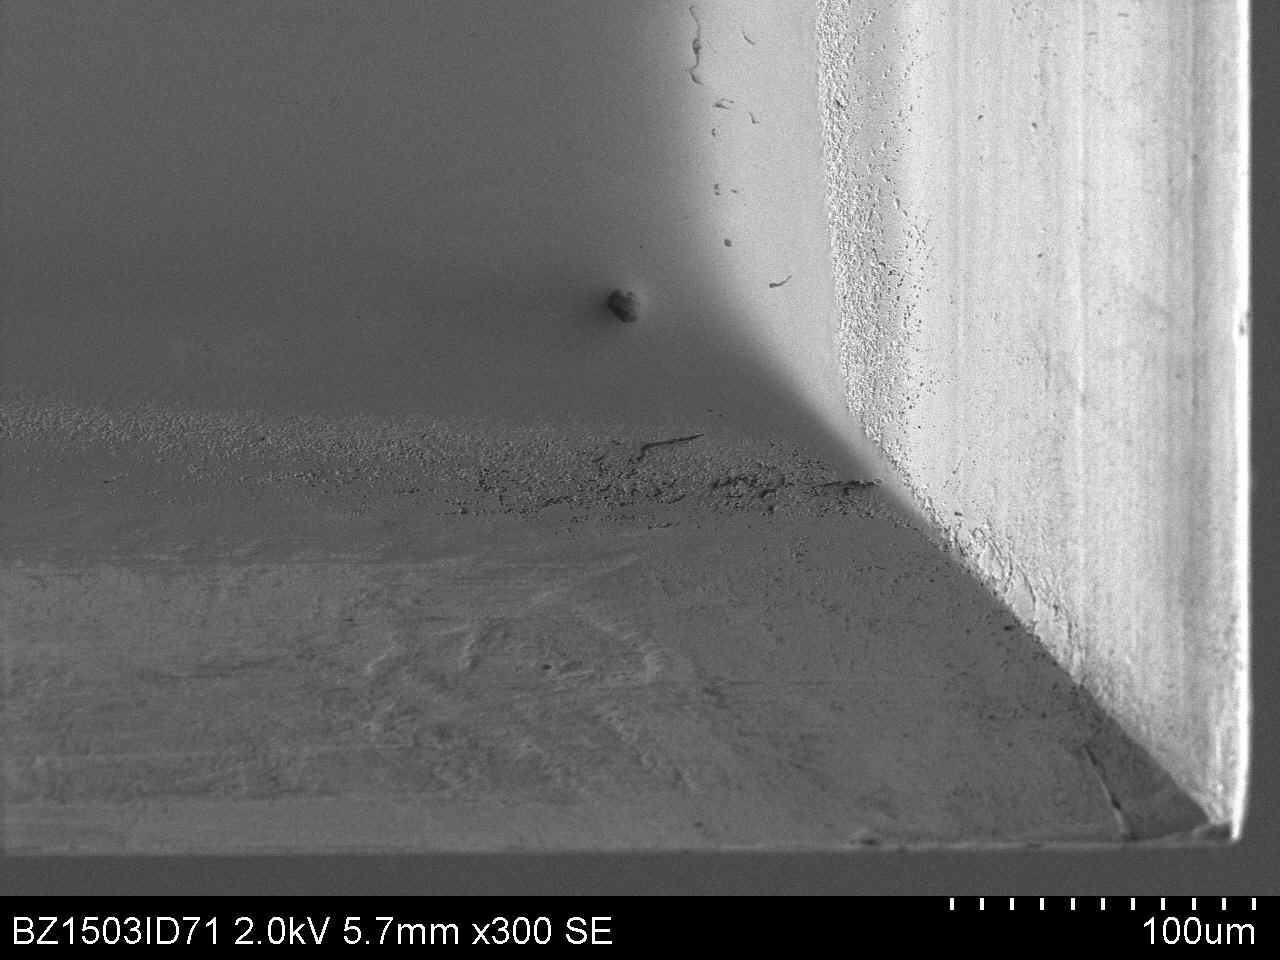
\includegraphics[width=0.48\linewidth]{SEM_BZ1503A_b_m008.jpg}}
    \quad
    \subfigure[SEM image of the southwest corner of substrate B at a magnification of 300$\times$.]{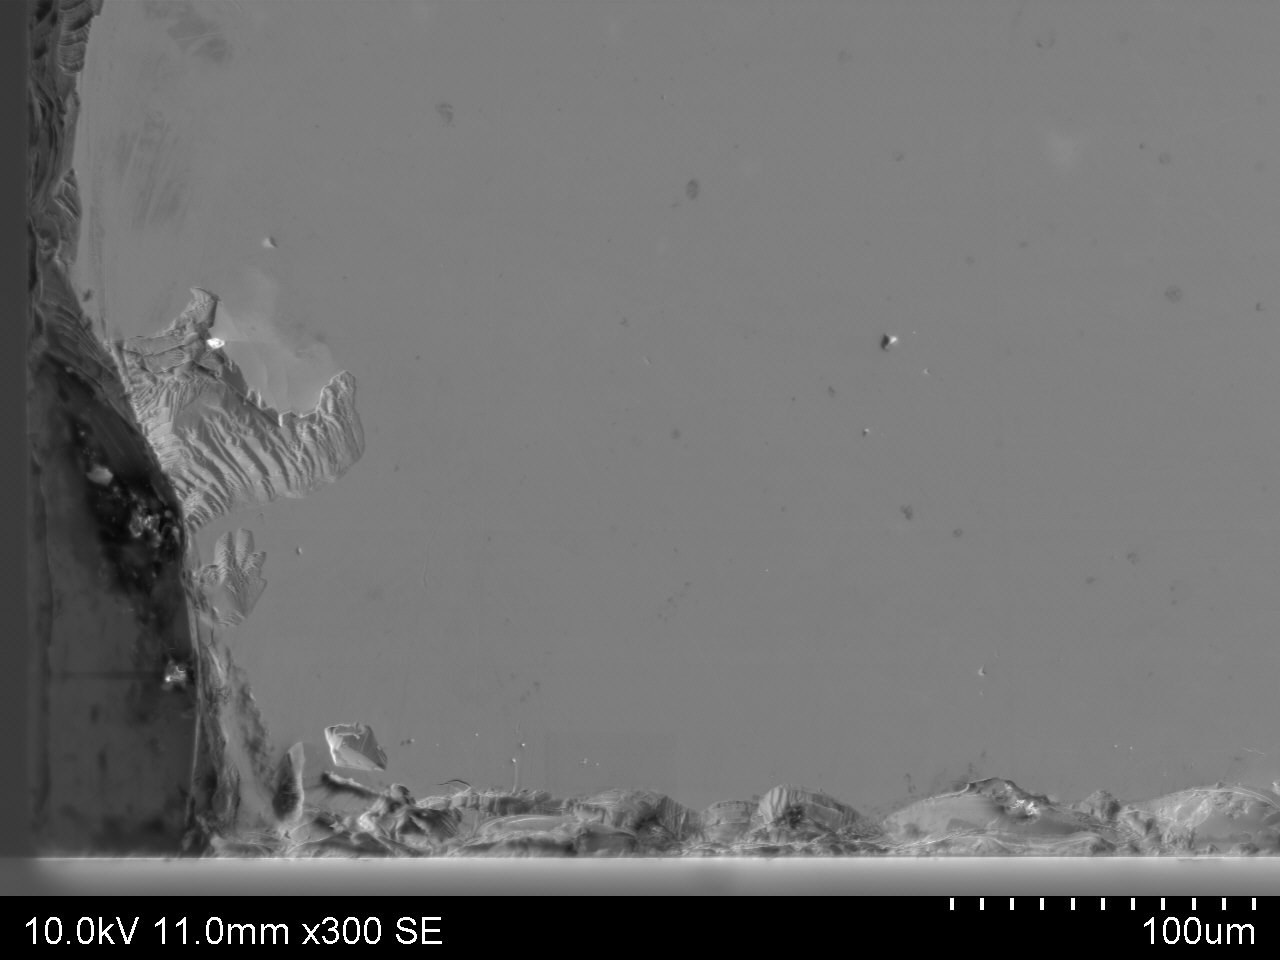
\includegraphics[width=0.48\linewidth]{20161214_C389523A_corners_m004.jpg}}
    \caption[SEM images of the corners on the substrates.]{Scanning electron microscopy (SEM) images of a corner on the two substrates taken at a magnification of 300$\times$.}
    \label{fig:SEM_corners}
\end{figure}


%%=========================================
\section{EDS Analysis of As-Received Substrates}

\Ac{eds} was performed on the substrates to determine the composition of the surface layers. Three areas on the substrates were analysed: the centre, \SI{1}{\milli\metre} from the centre of the upper edge, and \SI{1}{\milli\metre} from each of the edges of the the upper left corner. The analysis depth of \ac{eds} at \SI{12}{\kilo\volt} is about \SI{700}{\nano\metre}. As one monolayer of \ac{czt} is \SI{\sim 6.5}{\angstrom}, this implies that the result covers much more than the outermost surface layers. The quantitative result is an average elemental composition of the volume that is analysed.

\todo{Plasser et annet seted.} Ideally, \ac{xps} analysis, which has an analysis depth of \SI{\sim 80}{\angstrom} for \ac{mct}, should be performed on the substrates in order to determine the composition of the outermost layers of the substrates. Unfortunately, something was broken on the old analyser at \ac{ffi}, resulting in low signal intensity and no detection of impurities or small concentrations of elements. The ever-present oxide and carbon overlayers further decreased any small signals. Therefore, the XPS only gave information about the following elements: \ce{Te}, \ce{Cd}, \ce{O}, and \ce{C}. The reason for not performing \ac{xps} analysis on other than the as-received substrate A was that it would not be possible to detect the presence of impurities or small concentrations of elements with the \ac{xps} equipment at hand.

%\todo{Plagiat av meg selv?} The atomic concentrations was calculated using Eq.~\eqref{eq:xps_concentration} with intensity peak areas and the following experimentally measured atomic sensitivity factors, determined by \citet{hirsch1999x-ray}: \ce{Cd} 3d\textsubscript{5/2} (0.56), \ce{Te} 3d\textsubscript{5/2} (1.00), \ce{O} 1s (0.13), and \ce{C} 1s (0.05). Table~\ref{tab:xps_results} displays the results of the \ac{xps} analysis of the as-received substrate A. \ce{Cd_{0.96}Zn_{0.04}Te} should consist of \SI{48}{\atomic\percent} cadmium, \SI{2}{\atomic\percent} zinc and \SI{50}{\atomic\percent} tellurium, but zinc was not detected and the atomic concentration of \ce{Cd} was only \SI{75}{\percent} of that of \ce{Te} (it should be \SI{96}{\percent}). The higher than expected \ce{Te} concentration can be explained by the formation of a \ce{Te} oxide layer on the surface. By inserting the ratio between \ce{Te} in \ce{Cd_{1-y}Zn_yTe} signal and \ce{Te} in \ce{TeO} signal of \SI{1.3}{} into Eq.~\eqref{eq:signal_ratio}, the \ce{Te} oxide layer thickness was calculated to be \SI{0.96}{\nano\metre}. An atomic concentration of $23.5$ at.\% carbon was found, which can be explained by an overlayer of carbon.

%\todo{Plagiat av meg selv?}
Since the \ac{xps} equipment did not detect small concentrations of elements, \ac{eds} was used to get a quantitative analysis of the chemical composition of the substrate. The spectra were taken using an accelerating voltage of \SI{12.0}{\kilo\volt}, an extraction voltage of \SI{2.00}{\kilo\volt}, a large probe current, and the live acquisition time was set to \SI{1200}{\second} to get good statistics. The results of the \ac{eds} impurity analysis on the as-received substrates A, B, and C can be seen in Tables~\ref{tab:subAa_eds_analysis}, \ref{tab:subBa_eds_analysis}, and \ref{tab:subCa_eds_analysis} respectively. While the results of the \ac{eds} impurity analysis on the substrates after they were subjected to preparation etch, and polishing in the case of substrate C, can be seen in Tables~\ref{tab:subAb_eds_analysis}, \ref{tab:subBb_eds_analysis}, and \ref{tab:subCb_eds_analysis}.

%\todo{Plagiat av meg selv?}The electron interaction depth was calculated by the Quantax software to be \SI{0.4}{\micro\metre}. That means that characteristic x-rays from elements as far in as \SI{0.4}{\micro\metre} below the surface were detected. In comparison, the \ac{xps} detects the electrons that escape from the outermost \SI{\sim10}{\nano\metre}. Hence, \ac{eds} is not as surface sensitive and more than just the top surface layer is probed. This is the reason for the difference in the atomic concentrations between the \ac{xps} and \ac{eds} results for the as-received substrate A. The observed silica and alumina particles have a diameter of about \SI{50}{\nano\metre}. Hence, one layer of these would only cover \SI{12.5}{\percent} of the interaction volume.

%\todo{Plagiat av meg selv?} The \ac{eds} surface analysis identified the following elements on both of the substrates: \ce{Cd}, \ce{Te}, \ce{Zn}, \ce{Al}, \ce{Si}, \ce{C}, and \ce{O}. The relative concentrations of \ce{Cd}, \ce{Zn}, and \ce{Te} had an error of less than one percentage point from the expected value of \SI{48}{\atomic\percent} cadmium, \SI{2}{\atomic\percent} zinc and \SI{50}{\atomic\percent} tellurium. Substrate A had a smaller atomic concentration of \ce{O} than substrate B, which indicates that the tellurium oxide layer on substrate A was thinner than that on substrate B. The \ce{Al} and \ce{Si} contamination found in the \ac{eds} analysis for both substrate A and substrate B was coming from residual \ce{Al2O3} and \ce{SiO2} polishing grit respectively.

%%=========================================

\begin{table}[htbp]
    \centering
    \caption[\Ac{rms} roughness of the substrates.]{}\label{tab:sub_rms-roughness}
    \begin{tabu} to 1.0\textwidth { X[3,r] X[1,c] X[1,c] X[1,c] }
    \hline
                                & \textbf{Centre}  & \textbf{Edge}    & \textbf{Corner}    \\
        \hline
        As-received substrate A & \SI{}{} & \SI{}{} & \SI{}{}   \\
        As-received substrate B & \SI{}{} & \SI{}{} & \SI{}{}   \\
        As-received substrate C & \SI{}{} & \SI{}{} & \SI{}{}   \\
        \hline
        Etched substrate A      & \SI{}{} & \SI{}{} & \SI{}{}   \\  
        Polished and etched substrate B & \SI{}{} & \SI{}{} & \SI{}{}   \\  
        Etched substrate C      & \SI{}{} & \SI{}{} & \SI{}{}   \\  
        \hline
    \end{tabu}
\end{table}

%%=========================================